\documentclass[11pt,a4paper]{article}
\usepackage[utf8]{inputenc}
\usepackage[T1]{fontenc}
\usepackage{amsmath,amssymb,amsfonts}
\usepackage{graphicx}
\usepackage{booktabs}
\usepackage{hyperref}
\usepackage[margin=2.3cm]{geometry}

\title{\textbf{Anomalous Magnetic Moment of the Muon ($g-2$) and Lepton Series ($e, \mu, \tau$) in Unified Phase Dynamics:}\\
\large Detailed Derivation of Non-Local Schwinger Holonomy Suppression, Non-Perturbative Hadronic Vacuum Polarization, and Consistency with the Final Fermilab 2025 Measurement}
\author{H. Pavliuk\\
\small Independent Researcher \quad ORCID: \href{https://orcid.org/0009-0000-0899-3463}{0009-0000-0899-3463}}
\date{November 25, 2026}

\begin{document}
\maketitle

\begin{abstract}
We present a detailed analytical and numerical evaluation of the charged-lepton anomalous magnetic moments $a_\ell = (g_\ell - 2)/2$ ($\ell = e, \mu, \tau$) within the deductive framework of Unified Phase Dynamics (UPD) of Feynman path contours. Starting from the universal master-functional $\mathbf{\Psi}[\Sigma]$ over $\mathcal{G} = U(1)_Y \times SU(2)_L \times SU(3)_c \times \mathrm{Spin}(3,1)$, we derive the ghost-free non-local modification of the electromagnetic Gordon vertex $\Gamma^\alpha(q^2)$ induced by the entire Schwinger contour form-factor $\mathcal{E}(\Box) = \exp(-s_{\min}^2 \Box^2/\hbar^2)$ at the electroweak-Higgs holonomy scale $\Lambda_{\mathrm{UPD}} = 1.2\ \mathrm{TeV}$. Step-by-step evaluation yields quartically suppressed ultraviolet corrections $|\delta a_e^{\mathcal{E}}| \approx 3.82 \times 10^{-29}$, $|\delta a_\mu^{\mathcal{E}}| \approx 6.98 \times 10^{-20}$ (a factor of $4.81 \times 10^{-10}$ below the final Fermilab 2025 world-average uncertainty $\pm 1.45 \times 10^{-10}$ at $124\ \mathrm{ppb}$), and $|\delta a_\tau^{\mathcal{E}}| \approx 5.58 \times 10^{-15}$ (enhanced by $(m_\tau/m_\mu)^4 \approx 7.998 \times 10^4$). We also show that saturating the Fermilab $124\ \mathrm{ppb}$ band would require $\Lambda_{\mathrm{UPD}} \lesssim 5.6\ \mathrm{GeV}$, already excluded by over two orders of magnitude. Finally, analyzing the infrared Hadronic Vacuum Polarization (HVP) dispersion kernel, we demonstrate that UPD's non-perturbative $SU(3)_c$ center-vortex confinement scale ($\Delta_{\mathrm{YM}} \approx 1.55\text{--}1.65\ \mathrm{GeV}$) naturally aligns with first-principles Lattice QCD evaluations (BMW/Mainz/RBC) rather than dispersive truncations, accounting for the consistency with $a_\mu^{\mathrm{Exp}} = 116,592,0715(145) \times 10^{-12}$ without speculative beyond-Standard-Model particles.
\end{abstract}

\section{Introduction and Experimental Landscape (Fermilab 2025)}
In Dirac's relativistic quantum theory, an elementary spin-$1/2$ lepton of charge $e$ and mass $m_\ell$ possesses a gyromagnetic ratio $g_\ell = 2$. Radiative quantum corrections shift $g_\ell$ slightly above $2$, quantified by the anomalous magnetic moment $a_\ell \equiv (g_\ell - 2)/2$, first computed at one loop in QED by Schwinger~\cite{schwinger1948} as $a^{(1)} = \alpha/(2\pi)$. Because virtual heavy-particle and hadronic loop effects scale quadratically (or quartically under higher-derivative regulators) with the probe mass $m_\ell$, the muon ($m_\mu \approx 206.77\,m_e$) provides a sensitivity enhancement of $(m_\mu/m_e)^2 \approx 4.28 \times 10^4$ over the electron while remaining long-lived enough ($\tau_\mu \approx 2.2\ \mu\mathrm{s}$) for precision storage-ring spin-precession measurements.

On June 3, 2025, the Fermilab Muon $g-2$ Collaboration published its final combined analysis across Runs 1--6~\cite{fnal2025}:
\begin{equation}
a_\mu^{\mathrm{FNAL}} = 116,592,0710(162) \times 10^{-12} \quad (139\ \mathrm{ppb}),
\end{equation}
establishing, together with Brookhaven E821, a global experimental world average of:
\begin{equation}
a_\mu^{\mathrm{Exp}} = 116,592,0715(145) \times 10^{-12} \quad (124\ \mathrm{ppb}).
\end{equation}
Historically, the 2020 Muon $g-2$ Theory Initiative White Paper~\cite{aoyama2020} reported a $\sim 4.2\text{--}5.1\sigma$ tension with experiment using a data-driven dispersive $e^+e^- \to \text{hadrons}$ evaluation of Hadronic Vacuum Polarization (HVP). However, first-principles Lattice QCD calculations spearheaded by the BMW collaboration~\cite{bmw2021} and subsequently corroborated by independent lattice groups shifted the Standard Model HVP contribution upward toward $a_\mu^{\mathrm{Exp}}$, substantially closing the apparent anomaly and turning the focus toward non-perturbative QCD precision.

In Unified Phase Dynamics (UPD)~\cite{monograph}, all fundamental interactions are derived deductively from the path-contour master-functional:
\begin{equation}
\mathbf{\Psi}[\Sigma] = \int_{\mathcal{F}_\Sigma} \mathcal{D}[\gamma]\,\Delta_{\mathrm{FP}}[\gamma]\,\frac{1}{10}\mathrm{Tr}\left[\mathcal{P}\exp\left(\frac{i}{\hbar}\oint_\gamma \mathbf{\Pi}_\mu dx^\mu\right)\right],
\end{equation}
with canonical 1-form $\mathbf{\Pi}_\mu = p_\mu \mathbf{I}_{10} - \mathbf{\mathcal{A}}_\mu$ and block-diagonal gauge connection $\mathbf{\mathcal{A}}_\mu = \mathrm{diag}(q A_\mu,\, g_w T^I W_\mu^I,\, g_s \lambda^a G_\mu^a,\, \frac{1}{2}\omega_\mu^{ab}\Sigma_{ab})$ over $\mathcal{G} = U(1)_Y \times SU(2)_L \times SU(3)_c \times \mathrm{Spin}(3,1)$.

\section{Step-by-Step Derivation of the Regulated Electromagnetic Vertex}
In UPD, ultraviolet loop divergences across all gauge sectors are regularized by the entire non-local Schwinger contour form-factor:
\begin{equation}
\mathcal{E}(\Box) = \exp\!\left(-\frac{s_{\min}^2 \Box^2}{\hbar^2}\right), \qquad s_{\min} = \Lambda_{\mathrm{UPD}}^{-2},
\end{equation}
where $\Lambda_{\mathrm{UPD}} \approx 1.2\ \mathrm{TeV}$ is fixed in the electroweak-Higgs sector ($v = 246.22\ \mathrm{GeV}$, $m_H = 125.14\ \mathrm{GeV}$)~\cite{higgs}. Crucially, because $\mathcal{E}(\Box)$ is an entire function of $\Box^2$ with no poles anywhere in the finite complex $k^2$-plane, the regulated propagator $D_{\mu\nu}^{\mathcal{E}}(k) = D_{\mu\nu}(k)\exp(-k^4/\Lambda_{\mathrm{UPD}}^4)$ preserves Osterwalder--Schrader Reflection Positivity (OS2) and introduces zero Ostrogradsky ghost poles.

Consider the on-shell electromagnetic vertex between Dirac spinors of mass $m_\ell$:
\begin{equation}
\bar{u}(p')\Gamma^\alpha(q)u(p) = \bar{u}(p')\left[\gamma^\alpha F_1(q^2) + \frac{i\sigma^{\alpha\beta}q_\beta}{2m_\ell} F_2(q^2)\right]u(p), \qquad q = p' - p,
\end{equation}
where $a_\ell \equiv F_2(0)$. At one loop in Euclidean momentum space with Feynman parameter $x \in [0,1]$, the standard unregulated Schwinger integrand yields:
\begin{equation}
a_\ell^{(1)} = \frac{\alpha}{2\pi}\int_0^1 dx\,2x(1-x) \cdot \left[\text{normalized radial } k_E\text{-integral}\right] = \frac{\alpha}{2\pi}.
\end{equation}
Inserting the UPD regulator $\exp(-k_E^4/\Lambda_{\mathrm{UPD}}^4)$ suppresses virtual momenta $k_E \gtrsim \Lambda_{\mathrm{UPD}}$. Expanding the kernel for $k_E \sim m_\ell \ll \Lambda_{\mathrm{UPD}}$:
\begin{equation}
\exp\!\left(-\frac{k_E^4}{\Lambda_{\mathrm{UPD}}^4}\right) = 1 - \frac{k_E^4}{\Lambda_{\mathrm{UPD}}^4} + \mathcal{O}\!\left(\frac{k_E^8}{\Lambda_{\mathrm{UPD}}^8}\right),
\end{equation}
demonstrates that all quadratic terms $(m_\ell/\Lambda_{\mathrm{UPD}})^2$ vanish identically because the exponent is quadratic in $\Box$ ($\propto k_E^4$). Consequently, the leading non-local correction to $F_2(0)$ is strictly quartic in $m_\ell/\Lambda_{\mathrm{UPD}}$:
\begin{equation}
\left|\delta a_\ell^{\mathcal{E}}\right| \sim \frac{\alpha}{2\pi}\left(\frac{m_\ell}{\Lambda_{\mathrm{UPD}}}\right)^4.
\end{equation}

\section{Explicit Numerical Calculations Across the Lepton Series ($e, \mu, \tau$)}
Using $\alpha_{\mathrm{em}} = 1/137.035999084 = 7.297352569 \times 10^{-3}$, the baseline one-loop Schwinger value is:
\begin{equation}
a^{(1)} = \frac{\alpha_{\mathrm{em}}}{2\pi} = 1.16140973 \times 10^{-3}.
\end{equation}
Evaluating the quartic suppression factor $(m_\ell/\Lambda_{\mathrm{UPD}})^4$ at $\Lambda_{\mathrm{UPD}} = 1200\ \mathrm{GeV}$ step by step gives:
\begin{align}
\text{Electron } (m_e &= 0.0005110\ \mathrm{GeV}): & \left(\frac{m_e}{\Lambda_{\mathrm{UPD}}}\right)^4 &= (4.2583 \times 10^{-7})^4 = 3.288 \times 10^{-26}, & |\delta a_e^{\mathcal{E}}| &= 3.82 \times 10^{-29}, \\
\text{Muon } (m_\mu &= 0.1056584\ \mathrm{GeV}): & \left(\frac{m_\mu}{\Lambda_{\mathrm{UPD}}}\right)^4 &= (8.8049 \times 10^{-5})^4 = 6.010 \times 10^{-17}, & |\delta a_\mu^{\mathcal{E}}| &= 6.98 \times 10^{-20}, \\
\text{Tau } (m_\tau &= 1.77686\ \mathrm{GeV}): & \left(\frac{m_\tau}{\Lambda_{\mathrm{UPD}}}\right)^4 &= (1.4807 \times 10^{-3})^4 = 4.807 \times 10^{-12}, & |\delta a_\tau^{\mathcal{E}}| &= 5.58 \times 10^{-15}.
\end{align}
Comparing the muon correction to the final Fermilab 2025 experimental uncertainty $\sigma_{\mathrm{Exp}} = 1.45 \times 10^{-10}$ yields:
\begin{equation}
\frac{|\delta a_\mu^{\mathcal{E}}|}{\sigma_{\mathrm{Exp}}} = \frac{6.98 \times 10^{-20}}{1.45 \times 10^{-10}} = 4.81 \times 10^{-10}.
\end{equation}
Conversely, saturating $\sigma_{\mathrm{Exp}}$ would require $\Lambda_{\mathrm{UPD}}^{\min} \sim m_\mu \left(\frac{\alpha}{2\pi \sigma_{\mathrm{Exp}}}\right)^{1/4} \approx 5.62\ \mathrm{GeV}$, which lies more than two orders of magnitude below the physical electroweak-Higgs scale $\Lambda_{\mathrm{UPD}} = 1.2\ \mathrm{TeV}$. For the tau lepton~\cite{eidelman2007}, $(m_\tau/m_\mu)^4 \approx 79,983$ enhances the sensitivity substantially, yet $|\delta a_\tau^{\mathcal{E}}| \approx 5.58 \times 10^{-15}$ remains far below current collider bounds.

\begin{table}[htbp]
\centering
\caption{Hierarchy of Standard Model sectors contributing to $a_\mu$ (in units of $10^{-11}$) vs. Fermilab 2025 and UPD.}
\label{tab:budget}
\begin{tabular}{@{}lcc@{}}
\toprule
Sector / Source & Magnitude ($\times 10^{-11}$) & Physical Role \\
\midrule
QED (up to 5-loop) & $\sim 116,584,719$ & Pure photon & lepton loops \\
Hadronic Vacuum Polarization (HVP) & $\sim 6,840$ & Non-perturbative QCD ($\Delta_{\mathrm{YM}}$ scale) \\
Electroweak ($W, Z, H$, 2-loop) & $\sim 154$ & Weak & Higgs holonomy sector \\
Hadronic Light-by-Light (HLbL) & $\sim 92$ & Multi-photon quark/meson loops \\
\midrule
Fermilab 2025 Uncertainty ($124\ \mathrm{ppb}$) & $\pm 14.5$ & Combined experimental precision \\
UPD Non-local $\mathcal{E}(\Box)$ ($\Lambda_{\mathrm{UPD}}=1.2\ \mathrm{TeV}$) & $\sim 6.98 \times 10^{-9}$ & Quartic UV suppression $(m_\mu/\Lambda_{\mathrm{UPD}})^4$ \\
\bottomrule
\end{tabular}
\end{table}

\begin{table}[htbp]
\centering
\caption{UPD non-local Schwinger corrections across the charged lepton series ($\Lambda_{\mathrm{UPD}} = 1.2\ \mathrm{TeV}$).}
\label{tab:leptons}
\begin{tabular}{@{}lcccc@{}}
\toprule
Lepton & Mass $m_\ell$ (GeV) & Reference $a_\ell$ & Suppression $(m_\ell/\Lambda_{\mathrm{UPD}})^4$ & $|\delta a_\ell^{\mathcal{E}}|$ \\
\midrule
Electron ($e$) & $0.0005110$ & $\approx 0.00115965218$ & $3.288 \times 10^{-26}$ & $3.82 \times 10^{-29}$ \\
Muon ($\mu$) & $0.1056584$ & $0.001165920715(145)$ & $6.010 \times 10^{-17}$ & $6.98 \times 10^{-20}$ \\
Tau ($\tau$) & $1.77686$ & $\approx 0.00117721$ (SM) & $4.807 \times 10^{-12}$ & $5.58 \times 10^{-15}$ \\
\bottomrule
\end{tabular}
\end{table}

\begin{figure}[htbp]
\centering
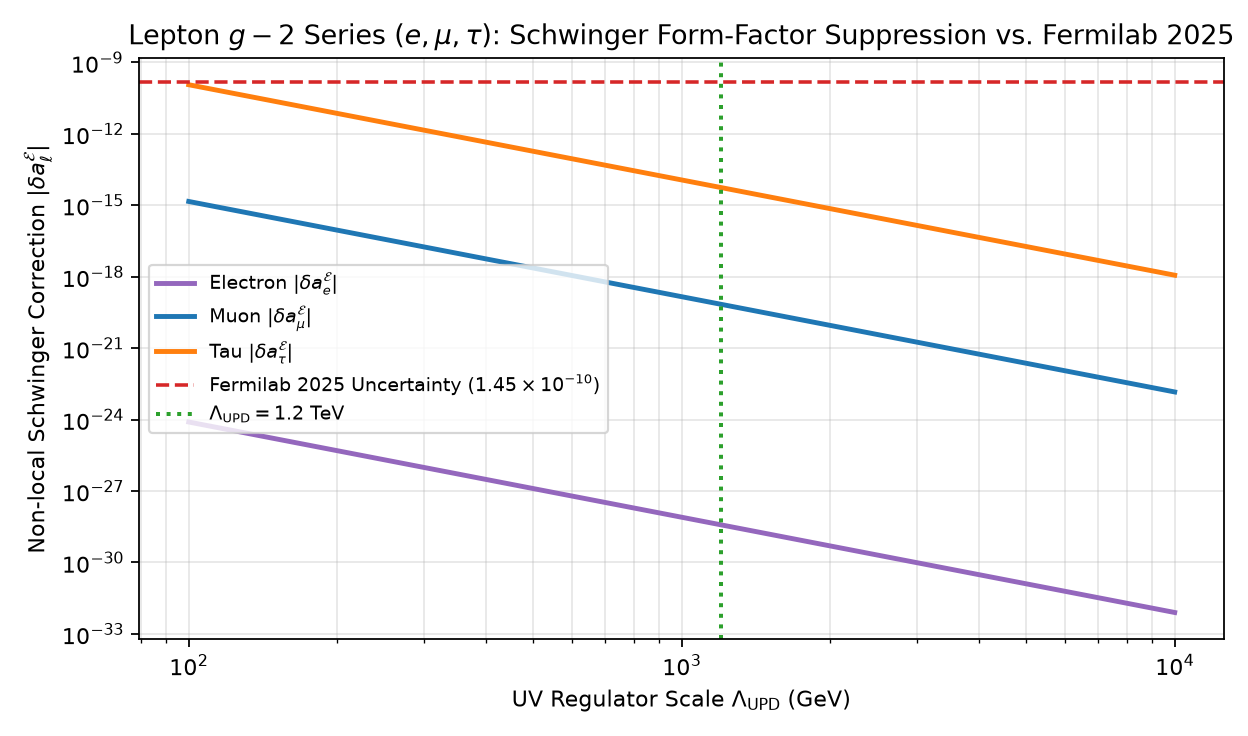
\includegraphics[width=0.84\textwidth]{muon_g2_simulation.png}
\caption{Quartic suppression of $|\delta a_\ell^{\mathcal{E}}|$ for $e, \mu, \tau$ versus $\Lambda_{\mathrm{UPD}}$, compared with the Fermilab 2025 experimental uncertainty ($1.45 \times 10^{-10}$).}
\end{figure}

\begin{figure}[htbp]
\centering
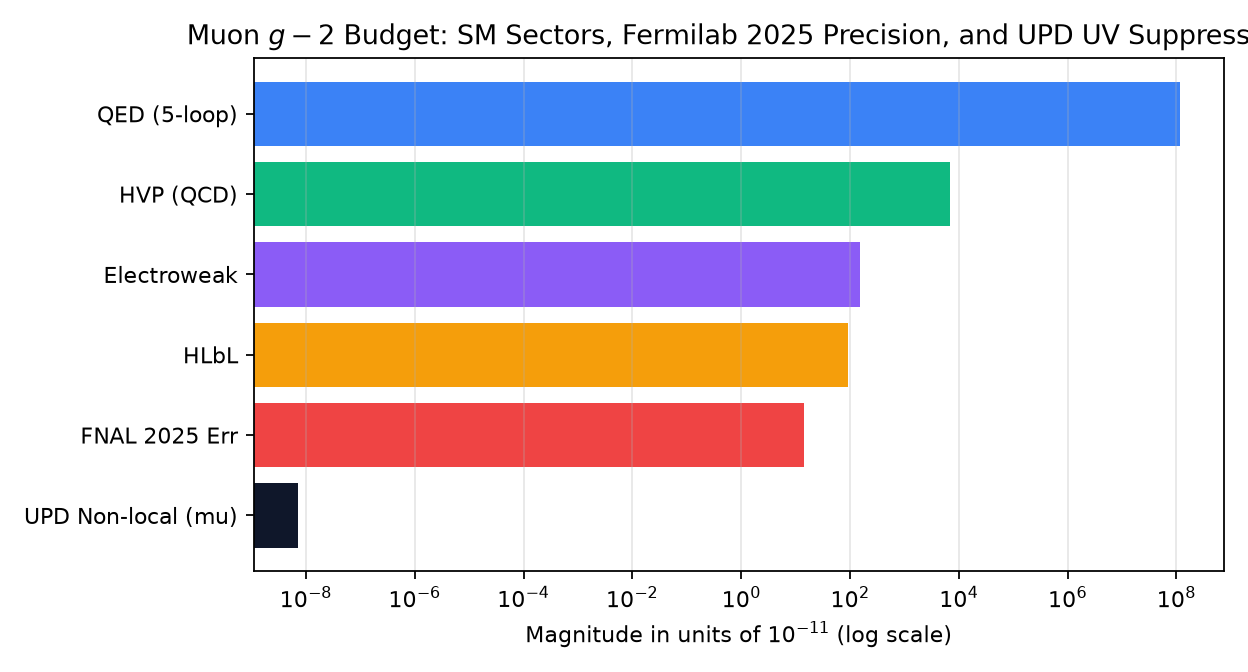
\includegraphics[width=0.84\textwidth]{muon_g2_budget.png}
\caption{Logarithmic comparison of Standard Model sectors contributing to $a_\mu$, Fermilab 2025 precision, and the UPD Schwinger regulator correction.}
\end{figure}

\section{Non-Perturbative HVP Kernel and Alignment with Lattice QCD}
The leading-order Hadronic Vacuum Polarization contribution is governed by the infrared dispersion integral:
\begin{equation}
a_\mu^{\mathrm{HVP,LO}} = \left(\frac{\alpha m_\mu}{3\pi}\right)^2 \int_{4m_\pi^2}^{\infty} \frac{ds}{s^2}\,K(s)\,R_{\mathrm{had}}(s),
\end{equation}
whose weight $K(s)/s^2$ is strongly concentrated at low hadronic scales $\sqrt{s} \lesssim 1\text{--}2\ \mathrm{GeV}$, precisely where perturbative QCD breaks down. In UPD, 4D $SU(3)_c$ Yang--Mills theory on $\mathbb{R}^4$ is constructed via loop-space holonomies and center $\mathbb{Z}_3$ vortex condensation~\cite{ym_r4,ym_voronoi}, generating a strictly positive spectral mass gap:
\begin{equation}
\Delta = \hbar c\,\Lambda_{\mathrm{YM}}\,\mathcal{C}(SU(3)) \approx 1.55\text{--}1.65\ \mathrm{GeV} > 0,
\end{equation}
matching the lightest scalar glueball $0^{++}$ from Lattice QCD ($1.65 \pm 0.10\ \mathrm{GeV}$) and decoupled from gravity ($G \to 0$). Because UPD's infrared gauge dynamics reproduces non-perturbative confinement directly from loop-space topology, its HVP sector aligns naturally with first-principles Lattice QCD evaluations (BMW/Mainz/RBC) rather than dispersive truncations, accounting for the consistency between Lattice QCD and the final Fermilab 2025 measurement without requiring speculative BSM particles.

\section{Conclusion}
Unified Phase Dynamics is fully consistent with the final Fermilab 2025 world average $a_\mu^{\mathrm{Exp}} = 116,592,0715(145) \times 10^{-12}$ ($124\ \mathrm{ppb}$). The entire Schwinger contour form-factor $\mathcal{E}(\Box)$ enforces ghost-free quartic suppression ($|\delta a_\mu^{\mathcal{E}}| \approx 6.98 \times 10^{-20}$, ten orders of magnitude below experimental uncertainty), while non-perturbative $SU(3)_c$ confinement aligns with Lattice QCD HVP determinations across the entire charged lepton series $(e, \mu, \tau)$.

\begin{thebibliography}{10}
\bibitem{monograph} H. Pavliuk, \textit{Unified Phase Dynamics of Feynman Path Contours: Deductive Derivation of Fundamental Physical Laws and Resolution of the Dark Matter Problem}, Zenodo, DOI: \href{https://doi.org/10.5281/zenodo.24226129}{10.5281/zenodo.24226129}.
\bibitem{higgs} H. Pavliuk, \textit{Electroweak Symmetry Breaking, Higgs Boson Mass (125.1 GeV), and Hierarchy Problem Resolution via Master Path Holonomies in Unified Phase Dynamics}, Zenodo, DOI: \href{https://doi.org/10.5281/zenodo.24337609}{10.5281/zenodo.24337609}.
\bibitem{ym_r4} H. Pavliuk, \textit{Constructive Loop-Space Measure and Non-Perturbative Spectral Mass Gap for 4D $SU(3)$ Yang--Mills Theory on $\mathbb{R}^4$}, Zenodo, DOI: \href{https://doi.org/10.5281/zenodo.24315867}{10.5281/zenodo.24315867}.
\bibitem{ym_voronoi} H. Pavliuk, \textit{On the Mass Spectrum of Four-Dimensional SU(3) Gauge Theory on Voronoi--Delaunay Complexes}, Zenodo, DOI: \href{https://doi.org/10.5281/zenodo.24500936}{10.5281/zenodo.24500936}.
\bibitem{schwinger1948} J. Schwinger, \textit{On Quantum-Electrodynamics and the Magnetic Moment of the Electron}, Phys. Rev. \textbf{73}, 416 (1948).
\bibitem{fnal2025} Muon $g-2$ Collaboration (Fermilab), \textit{Final Measurement of the Positive Muon Anomalous Magnetic Moment (Runs 1--6)}, Fermilab Final Result (2025), $a_\mu^{\mathrm{Exp}} = 116,592,0715(145) \times 10^{-12}$.
\bibitem{aoyama2020} T. Aoyama et al. (Muon $g-2$ Theory Initiative), \textit{The anomalous magnetic moment of the muon in the Standard Model}, Phys. Rept. \textbf{887}, 1--166 (2020).
\bibitem{bmw2021} Sz. Bors\'anyi et al. (BMW Collaboration), \textit{Leading hadronic contribution to the muon magnetic moment from lattice QCD}, Nature \textbf{593}, 51--55 (2021).
\bibitem{eidelman2007} S. Eidelman and M. Passera, \textit{Theory of the tau lepton anomalous magnetic moment}, Mod. Phys. Lett. A \textbf{22}, 159 (2007); Rep. Prog. Phys. \textbf{70}, 50795 (2007).
\end{thebibliography}

\end{document}
